\documentclass[twocolumns]{IEEEtran}
\usepackage[utf8]{inputenc}
\usepackage[linesnumbered,lined, algoruled]{algorithm2e}
\usepackage{algorithmic,float}
\usepackage{amsmath}
\usepackage{amsthm}
\usepackage{amsfonts}
\usepackage{amssymb}
\usepackage{balance}
\usepackage{bm,array}
\usepackage{color,soul}
%\usepackage{epstopdf}
\usepackage[acronym,shortcuts]{glossaries}
\usepackage{graphicx}
\usepackage{graphics}
\usepackage[inline]{enumitem}
\makeglossaries
%%% Glossaries/Acronyms


\newacronym{auc}{AUC}{area under the curve}
\newacronym{bs}{AP}{access point}
\newacronym{ce}{CE}{cross entropy}
\newacronym{fa}{FA}{false alarm}
\newacronym{kl}{K-L}{Kullback-Leibler}
\newacronym{ls}{LS}{least-squares}
\newacronym{llr}{LLR}{log likelihood-ratio}
\newacronym{los}{LOS}{line of sight}
\newacronym{lssvm}{LS-SVM}{least squares SVM}
\newacronym{md}{MD}{mis-detection}
\newacronym{ml}{ML}{machine learning}
\newacronym{mlp}{MLP}{multy-layer perceptron}
\newacronym{mse}{MSE}{mean squared error}
\newacronym[\glslongpluralkey={neural networks}]{nn}{NN}{neural network}
\newacronym{np}{N-P}{Neyman-Pearson}
\newacronym{oclssvm}{OCLSSVM}{one-class least-square \ac{svm}}
\newacronym{pdf}{PDF}{probability distribution function}
\newacronym{pmd}{PMD}{probability mass distribution}
\newacronym{pso}{PSO}{particle swarm optimization}
\newacronym{rnn}{RNN}{replicator neural network}
\newacronym{roc}{ROC}{receiver operating characteristic}
\newacronym{rss}{RSS}{received signal strength}
\newacronym[\glslongpluralkey={support vector machines}]{svm}{SVM}{support vector machine}
\newacronym{ue}{UE}{user equipment}
\newacronym{wsn}{WSN}{wireless sensor network}
\newacronym{irlv}{IRLV}{in-region location verification}

%\usepackage[autostyle]{csquotes}
\usepackage[backend=biber,style=ieee]{biblatex}
\bibliography{bibliography}


\title{Location-Verification and Network Planning \\ via Machine Learning Approaches}
\author{Alessandro Brighente, Francesco Formaggio, Giorgio Maria Di Nunzio, and  Stefano Tomasin  \\ {\small Department of Information Engineering, University of Padova, via G. Gradenigo 6/B, Padova, Italy. first.lastname@dei.unipd.it} }
\date{today}

\begin{document}

\maketitle

\begin{abstract}
We consider the \ac{irlv} problem of deciding if a message coming from a terminal over a wireless network has been originated from a specific physical area (e.g., a safe room) or not. The detection process exploits the features of the channel over which the transmission occurs with respect to a set of network access points. A  \ac{ml} approach is used, based on  \ac{nn} or a \ac{svm} trained with channel features  (in particular, noisy attenuation factors) collected by the access points for various positions of the terminal both inside and outside the specific area. By seeing the \ac{irlv} problem as an hypothesis testing problem, we address the optimal positioning of the access points for maximizing either the \ac{auc} of the \ac{roc} or  the \ac{ce} between the decision variable and its correct value. Through simulations we show that for long training and machines with enough parameters the proposed solution achieves the performance of the \ac{np} lemma, and we apply a \ac{pso} approach for the optimization of the access point positions.
\end{abstract}

\begin{IEEEkeywords}
Physical layer security, location verification, neural network, support vector machine, network planning
\end{IEEEkeywords}
\glsresetall

\section{Introduction}

The applications exploiting the location of the user are rapidly spreading as they allow to provide very customized services, from shopping opportunities to proper data collection for sensor network. In some cases services should be available only pre-determined areas for commercial or legal reasons, e.g., media streaming, such as online voting, online gambling and location-based social networking. In these and other application it is important to verify the position of the user rather than simply rely on its claims, that can easily forged by hacking the software.

Location verification systems aims at verifying the position of a devices in a mobile communication network, and find application in various scenarios, spanning from sensor networks \cite{Zeng-survey, 8376254}, to the Internet of Things \cite{7903611}, to geo-specific encryption \cite{quaglia}. Various approaches have been proposed, typically based on the measurement of the distance between the transmitter and other users  or  anchor nodes belonging to the network infrastructure. The distance measures are obtained for example through the \ac{rss} at anchor nodes for signals transmitted by the terminal to be verified.  This problem is closely related to the {\em user authentication} at the physical layer, where the channel features are exploited to verify the sender of a message over a wireless channel \cite{7270404}.

In this paper we focus on the {\em in-region} location verification problem, i.e., the problem of deciding if a message coming from a terminal over a wireless network has been originated from a specific physical area (e.g., a safe room) or not \cite{quaglia}. This can be seen as an hypothesis testing problem between two alternatives, namely being inside or outside the specific area. Among proposed solutions we recall distance bounding techniques with rapid exchanges of packets between the verifier and the prover \cite{Brands}, also using radio-frequency and ultrasound signals \cite{Sastry}, and solutions based on the use of anchor nodes and increasing transmit power by the sender \cite{Vora}. More recently in \cite{7145434} a delay-based verification technique has been proposed, leveraging geometric properties of triangles, which prevents an adversary from manipulating measured delays.  

In this paper we consider the location verification problem exploiting the features of the channel over which the transmission occurs with respect to a set of network access points, and can be seen as a location-verification system. We start from the observation that as an hypothesis testing problem, the most powerful test for a given significance for \ac{irlv} is provided by the \ac{np} lemma \cite{Neyman289}, i.e., the test providing the minimum \ac{md} probability for a given \ac{fa} probability. We derive close-form expressions for the \ac{np} test for a simple channel model and simple access point configuration. Then we observe that for more complicated situations the close-form solution may not be available. Moreover,  channel impairments that affect the measurements may not be known statistically, as they may depend on random unknown phenomena as shadowing and fading. We therefore propose here to use a \ac{ml} approach, where first data are collected by trusted nodes both inside and outside the region of interest and a machine is trained to take decisions between the two hypothesis before deployment as tester. \ac{ml} techniques have already found application in the user authentication problem (see  \cite{pei2014channel, tian2015robust,Wang-17, xiao-2018, }). However, to the best of authors' knowledge \ac{ml} solutions have never been applied before to the \ac{irlv} problem. 

We design the \ac{ml} solutions using the \ac{ce} between the decision variable and its correct value as optimization criterion and we show by simulations that the \ac{roc} of the \ac{ml} detector converges to that of the \ac{np} test as the complexity of the machine grows, in terms of number of neurons or training set size, and the number of training points goes to infinity. We then address the problem of optimum positioning of the access points that provides the data over which the test is performed. Two metrics are considered: the \ac{ce} between the decision variable and its correct value and the \ac{auc} of the \ac{roc}. Both are known to provide a single-number indication on how good the tests is. In a simulation environment, a \ac{pso} solution is proposed to attractively update the position of the access points gradually increasing the target metrics until convergence to a local optimum. Multiple starting points are considered and the \ac{pso} is repeated in order to get closer to the global optimum position of the access points. We also show the relation between the two metrics, \ac{auc} and \ac{ce}, showing how both are function of the two test metrics, i.e., \ac{fa} and \ac{md} probabilities.

The rest of the paper is organized as follows \hl{TBD}

%Network planning, i.e., designing optimal \acp{bs}' layout maximizing a chosen metric, has been studied in the literature in the context of \ac{wsn} \cite{bogdanov2004power} \cite{akkaya2007positioning} and cellular systems \cite{mathar2001optimal} \cite{glasser2005complexity}  \cite{islam2012capacity} \cite{yangyang2004particle}. In \cite{bogdanov2004power} the sensors network is optimized using as metric the rate of transmission between nodes. The resulting optimization is then solved using two heuristic iterative algorithms, since the problem is NP-complete. For a comparison between other proposed approaches and metric choices for \ac{wsn}, see \cite{akkaya2007positioning}. For what concerns cellular systems, in \cite{mathar2001optimal} and \cite{islam2012capacity} the chosen metrics are, respectively, the number of connected users and the cumulative channel capacities. For both these works the solving tools are taken from the integer and mixed-integer programming literature. In \cite{yangyang2004particle}, instead, \ac{pso} is used to optimize \acp{bs}' position w.r.t coverage and deployment costs (proportional to  the number of \acp{bs}).
%To the best of authors' knowledge there are no literature examples of \acp{bs} positions planning that seek to optimize physical layer authentication performance.
 
\section{System Model}


We consider a cellular system with $N_{\rm BS}$ \acp{bs} covering a region $\mathcal{A}$ over a plane. We propose a location authentication system able to determine if a \ac{ue} is transmitting from within an {\em authorized} sub-region $\mathcal{A}_0$ of the region $\mathcal{A}$. The location dependency of the features of the channel between the \ac{ue} and the \acp{bs} is exploited to distinguish between a transmission from the region $\mathcal{A_0}$ and a transmission from the complementary region $\mathcal{A}_1=\mathcal{A} \setminus \mathcal{A}_0$. We consider here a narrowband transmission and we focus on the power received by the \acp{bs} upon \ac{ue} transmission.

The location authentication procedure is composed by two phases. In the first phase ( authentication identification) the \ac{ue} transmits a training signal ( known at the \acs{bs}) from various points within region $\mathcal{A}_0$, and the \acp{bs} estimates the attenuation value incurred by the transmitted signal and store them in association with $\mathcal{A}_0$. Some external authentication technique must be added in this phase in order to ensure that the \ac{ue} is transmitting from region $\mathcal{A}_0$. Similarly the \ac{ue} transmits a training signal from the complementary area $\mathcal{A}_1$ and the \acp{bs} estimate the attenuation value and store them in association to $\mathcal{A}_1$.

In the second phase (authentication verification) the \ac{ue} transmits a known training sequence from any points in $\mathcal{A}$, and the \acp{bs} must decide whether the \ac{ue} is in region $\mathcal{A}_0$ or $\mathcal{A}_1$.

The location dependency of the features of the transmission channel can be further enhanced by properly placing the \acp{bs} over the area $\mathcal{A}$. In particular, different positioning lead to different shadowing incurred by the transmission of the \acp{ue} toward the \acp{bs}. Our aim is to find the optimal \acp{bs} positioning such that the authentication system can optimally discriminate between different areas based on the estimated attenuation values.

\subsection{Channel Model}

Consider a network with $N_{\rm bs}$. We denote as $\bm{x}_{\rm bs}^{(n)} =(X_{\rm bs}^{(n)},Y_{\rm bs}^{(n)})$ the position of the $n^{\rm th}$ \ac{bs}. For a \ac{ue} located at $\bm{x}_{\rm ue}=(X_u,Y_u)$, its distance from \ac{bs} $n$ is
\begin{equation}
    L(\bm{x}_{\rm ue},\bm{x}_{\rm bs}^{(n)}) = \sqrt{(X_{\rm bs}^{(n)}-X_u)^2+(Y_{\rm bs}^{(n)}-Y_u)^2}.
\end{equation}
When a \ac{ue} transmits with power $P_{\rm tx}$, the received power at the $n^{\rm th}$ \ac{bs} is
\begin{equation}\label{eq: rec pow}
    P_{\rm rc}^{(n)}= \frac{P_{\rm tx}}{a^{(n)}},
\end{equation}
where $a^{(n)}$ is the attenuation incurred by the transmitted signal to \ac{bs} $n$. The attenuation coefficient $a^{(n)}$ includes the effects of path-loss, shadowing and fading. Denoting the path-loss coefficient as $P_{\ell}^{(n)}$ and as $s \sim \mathcal{N}(0,\sigma_s^2)$ the shadowing component we can define the fading power as $\sigma_{a,n}^2={P_{\ell}^{(n)}}e^{s}$. The fading realization is hence a zero mean $\sigma_{a,n}^2$ Gaussian random variable, i.e.,
\begin{equation}
    \sqrt{a^{(n)}} \sim \mathcal{N}\left(0,\sigma_{a,n}^2\right),
\end{equation}

The channel model for path loss and shadowing is the on in \cite{3gpp}. For the path-loss we consider two scenarios: \ac{los} and non-\ac{los}.

For a \ac{los} link the path loss coefficient in dB is modelled as
\begin{equation}\label{eq:los}
    P_{\ell,LOS}^{(n)} = 20\log_{10}\left(\frac{f 4\pi L(\bm{x}_{\rm ue},\bm{x}_{\rm bs}^{(n)})}{c}\right),
\end{equation}
where $f$ is the carrier frequency and $c$ is the speed of light.

For a  non-\ac{los} link the path loss coefficient in dB is defined as
\begin{equation}
\begin{split}
    P_{\ell, non-LOS}^{(n)} = 40\left(1-4\times 10^{-3}\times h_{\rm BS}\right)\log10\left (\frac{L(\bm{x}_{\rm ue},\bm{x}_{\rm bs}^{(n)})}{10^3}\right ) \\
    -18\log_{10}h_{\rm BS}
    + 21\log10\left(\frac{f}{10^6}\right) + 80,
    \end{split}
\end{equation}
where $h_{\rm SB}$ is the \ac{bs} antenna elevation.

We assume that shadowing is time-invariant while fading is time dependent. We also assume that shadowing $s$ depends on positions $\bm{x}_{\rm ue}$ and $\bm{x}_{\rm bs}^{(n)}$ and is correlated at different \ac{ue} and \ac{bs} positions. The shadowing map for the area is generated as a multivariate Gaussian distribution with correlation matrix $\bm{\Sigma}$ whose entry $\left[\bm{\Sigma}\right]_{(i,j)}$ is given by the covariance between two positions $\bm{x}_i$ and $\bm{x}_j$. This depends on their relative distance $d(\bm{x}_i,\bm{x}_j)$ as
\begin{equation}\label{eq: coor mat}
    \left[\bm{\Sigma}\right]_{(i,j)} = e^{-\frac{d}{d_c}},
\end{equation}
where $d_c$ is the shadowing decorrelation distance. 

\subsection{LOS Case}

In this section we derive the \ac{llr} function for a simplified scenario. We will use this result in the numerical section part to compare the classificator performance of the \ac{ml} approaches with the optimal one.

Let us define the overall network area as a circle $\mathcal{C}$ with radius $R_{\rm out}$ and consider a single \ac{bs} located at the center of $\mathcal{C}$. Consider the legitimate area $\mathcal{A}_{0}$ as a rectangle of height $H$ and length $L$ and with nearest point to the center of $\mathcal{C}$ at a distance $R_{\rm min}$. The non-legitimate area is $\mathcal{A}_1 = \mathcal{C} \setminus \mathcal{A}_0$.

Iin the \ac{los} scenario the attenuation incurred by a \ac{ue} only depends on its relative distance to the \ac{bs}. We can here compute the closed form \ac{llr} of the region dependent attenuation value probabilities $p(\bm{a}|\mathcal{H}_i)$ as
\begin{equation}\label{eq:lr}
    \mathcal{L}^{(\bm{a})}=\log\left(\frac{p(\bm{a}|\mathcal{H}_0)}{p(\bm{a}|\mathcal{H}_1)}\right).
\end{equation}

Consider a \ac{ue} $u$ transmitting a message to the \ac{bs} located at a distance $R_0$ from the \ac{bs}. The probability that $u$ is located at a distance $R\le R_0$ in $\mathcal{A}_0$ is
\begin{equation}\label{eq:cdf}
     \mathbb{P}(R \le R_0|\mathcal{A}_0) = \frac{1}{|\mathcal{A}_0|}\int_{R_{\rm min}}^{R_0} R a(R) dR,
\end{equation}
where $a(R)$ denotes the angle of the circular sector located at distance $R$ intersecting area $\mathcal{A}_0$.

By taking the derivative of (\ref{eq:cdf}) respect to $R_0$ we obtain the \ac{pdf} of $u$ transmitting from a distance $R_0$ given that it is located in $\mathcal{A}_0$ as
\begin{equation}
    p(R_0|\mathcal{A}_0) = \frac{1}{|\mathcal{A}_0|}R_0a(R_0).
\end{equation}
Following the same reasoning and considering that the length of the arc of circle with radius $R_0$ located in $\mathcal{A}_1$ is $2\pi - a(R_0)$, we obtain the \ac{pdf} of $u$ being at a distance $R_0$ given that it is located in $\mathcal{A}_1$ as
\begin{equation}
     p(R_0|\mathcal{A}_1) = \frac{1}{|\mathcal{A}_1|}R_0\left(2\pi-a(R_0)\right),
\end{equation}
from which we obtain the closed form solution for (\ref{eq:lr}) 
\begin{equation}
    \mathcal{L}=\log\left(\frac{|\mathcal{A}_1|a(R_0)}{|\mathcal{A}_0|\left(2\pi-a(R_0)\right)}\right).
\end{equation}

\section{Classification via Machine Learning}
In this section we quickly review two \ac{ml} techniques, namely the \ac{mlp} and the \ac{svm}, and show how to exploit them in order to perform user authentication.

We assume that the authentication system has access to both regions $\mathcal{A}_0$ and $\mathcal{A}_1$ and that during the authentication phase $S$ attenuation vectors $\bm{a}^{(i)}, \ i=1,\dots S$  belonging to both regions are collected. These values will then be used as input of the \ac{ml} algorithms. Denoting as $\bm{a}^{(i)}\in \mathcal{A}_n$ an attenuation vector generated from a \ac{ue} located in area $\mathcal{A}_{n}$, the objective is to obtain at the output of the \ac{ml} algorithm the identification function defined as
\begin{equation}
  t_i =
  \begin{cases}
  -1 \quad \text{if} \quad \bm{a}^{(i)} \in \mathcal{A}_0\\
  1 \quad \text{if} \quad \bm{a}^{(i)} \in \mathcal{A}_1.
  \end{cases}
\end{equation}
The vector $\bm{t}=[t_1,...,t_S]$ is defined as the vector of the labels of the attenuation vectors and will be used as training objective for the \ac{ml} approaches.

In order to test and compare the authentication systems we define two error probabilities: the \ac{fa} probability, i.e. the probability  that a legitimate user is classified as non-legitimate $P_{\rm FA} =P(\hat{\mathcal H} = \mathcal H_1 | \mathcal H_0)$; the \ac{md} probability, i.e., the probability that a non-legitimate user is classified as legitimate, $P_{\rm MD}=P(\hat{\mathcal H} = \mathcal H_0 | \mathcal H_1)$.

\subsection{Multi-Layer Perceptron}\label{sec:nn}

A \ac{mlp} is a feed-forward neural network which implements a function of the type $\mathbb{R}^N \to \mathbb{R}^O$, which maps a set of $N$ real values into $O$ real values. The input is processed in stages, named layers, where the output of one layer is the input of the next layer.

Layer $L-1$ has $N^{(\ell-1)}$ outputs obtained by processing the inputs with $N^{(\ell-1)}$ functions named neurons. The output of the $n^{\rm th}$ neuron of the $\ell^{\rm th}$ layer is
\begin{equation}\label{eq:nonLin}
y_n^{(\ell)} = \psi\left( \bm{w}_n^{(\ell -1)}\bm{y}^{(\ell-1)}+b_n^{(\ell)} \right),
\end{equation}
i.e., a mapping via an activation function $\psi$ of the weighted linear combination with weights $\bm{w}_n^{(\ell -1)}\in \mathbb{R}^{1\times N^{(\ell-1)}}$ of the outputs $\bm{y}^{(\ell-1)} \in \mathbb{R}^{N^{(\ell-1)} \times 1 }$ of the previous layer plus a bias $b_n^{(\ell)} \in \mathbb{R}^{N^{(\ell-1)} \times 1 }$. We denote respectively as $\bm{y}^{(0)}$ and $\bm{y}^{(L-1)}$ the input and the output of the \ac{mlp}. 

The \ac{mlp} must be properly trained in order to perform classification, i.e., the optimal values for the vectors $\bm{w}_n^{(\ell)}$ and the scalars $b_n^{(\ell)}$ must be computed. \Ac{mlp} training is performed via gradient descent minimizing the \ac{ce} defined as
\begin{equation}\label{eq:ce}
CE = -\sum_{i=1}^{S}\left(\tilde{y}_i\log\left(t_i\right)+\left(1-\tilde{y}_i\right)\log\left(1-t_i\right) \right),
\end{equation}
where $\tilde{y}_i$ denotes the output of the \ac{ce}-trained \ac {mlp} when the input is $\bm{a}^{(i)}$.

Since the output of the neural network $y^{(L-1)}$ is a continuous value in $[-1,1]$, in order to perform classification, a suitable threshold value $\lambda$ must be chosen, such that the input vector $\bm{y}^{(0)}$ is classified as
$\mathcal{H}_0$ if $\bm{y}^{(L-1)} > \lambda$ and as $\mathcal{H}_1$ if $\bm{y}^{(L-1)} \le \lambda$.

\subsection{Support Vector Machine}\label{sec:svm}
A \ac{svm} \cite{Bishop2006} is a supervised learning model that can be used for classification and regression. We focus here on binary classification, i.e., given the input vector $\bm{y}^{(0)} \in \mathbb{R}^N$ the \ac{svm} returns $\hat{t} = 1$ if $\bm{y}^{(0)}$ belongs to class 0 whereas $\hat{t}=-1$ if $\bm{y}^{(0)}$ belongs to class 1. It comprises the function $\tilde{t}: \mathbb{R}^N \to \mathbb{R}$ defined by
\begin{equation}
\label{eq:svm}
\tilde{t} = \mathbf{w}^T \phi (\mathbf{a}^{(i)}) + b,
\end{equation}
where $\phi: \mathbb{R}^N \to \mathbb{R}^K$ is a feature-space transformation function, $\mathbf{w} \in \mathbb{R}^K$ is the weight vector and $b$ is a bias parameter, and the decision function is
\begin{equation}
\label{eq:cases}
\hat{t} = 
\begin{cases}
+1 \quad \tilde{t}  \geq \gamma^* \\
-1 \quad \tilde{t}  < \gamma^*,
\end{cases}		
\end{equation} 
where $\gamma^*$ is a fixed threshold and controls \ac{fa} and \ac{md} probabilities. Note that in the classical \ac{svm} formulation we have $\gamma^* = 0$.

While the feature-space transformation function is typically fixed, the vector $\mathbf{w}$ must be properly chosen to perform the desired classification


\section{APs' Optimal Position}\label{sec:bsPos}



As attenuation maps depend on the position of the \acp{bs} and on the surrounding environment in terms of shadowing effects the performance of the authentication system depend on the number of \acp{bs} and their location in the space. In this section we derive an approach to optimally locate \acp{bs} so that the authentication system attains the best performance. 

A performance metric to be minimized for the optimization of \ac{bs} position could be the \ac{md} probability for a fixed \ac{fa} probability. However, for different values of target \ac{fa} probability we should re-optimize the \ac{bs} position. Here we focus instead on metrics independent from specific values of the \ac{fa} probability, i.e., that depends on the \ac{roc} as a whole. Note that in this paper we consider the \ac{roc} as the \ac{md} probability as a function of the \ac{fa} probability. The \ac{roc} can be obtained by training the detectors and then computing the \ac{fa} and \ac{md} probabilities for all possible values of thresholds \hl{TBD}, for \ac{nn} and \ac{svm}. In particular, we consider two metrics, i.e., the   \ac{roc} \ac{auc} \cite{hanley-82} and the  \ac{ce}.

The \ac{roc} \ac{auc} is defined as 
\begin{equation}
    \text{\ac{auc}}(\mathcal{X}) = \int_{0}^{1} P_{\rm MD}\left(P_{\rm FA}\right) d P_{\rm FA},
\end{equation}
where $P_{\rm MD}\left(P_{\rm FA}\right)$ is the $P_{\rm MD}$ value as a function of the $P_{\rm FA}$, which correspond to the integral of the \ac{roc} function. By minimizing the \ac{auc} we minimize the average \ac{md} probability for a uniform \ac{fa} probability\footnote{Notice that traditionally the \ac{auc} is a metric that needs to be maximized \cite{hanley-82}. This is due to the fact that the curve of the system performance computed as in \cite{hanley-82} and \cite{Kennedy-11} is given by the true positive rate vs. the false negative rate value, which is optimal when the true positive rate value is maximized for each false negative rate value. Since we consider as system performance metrics for the authentication system the $P_{\rm MD}$ and the $P_{\rm FA}$ we instead need to minimize the \ac{auc}.}. 

The \ac{ce} is defined in (\ref{eq:ce}), which can also written as 
\begin{equation}
\mathbb H(p_t,p_{\hat{t}}) = \mathbb H(p_t) + \mathbb D(p_t; p_{\hat{t}})\,,
\end{equation}
where $p_t$ is the \ac{pmd} of $t$, $p_{\hat{t}}$ is the \ac{pmd} of $\hat{t}$, $\mathbb H(\cdot)$ is the entropy function and $\mathbb D(\cdot;\cdot)$ is the Kullback-Leibler divergence which for Bernoulli variables can be written as 
\begin{equation}
\mathbb D(p_t; p_{\hat{t}}) = 
\end{equation}

and by the definition of entropy and Kullback-Leibler divergence between two random varia

However the computation of the \ac{auc} implies that for each \acp{bs} setting we must train and test a \ac{ml} algorithm, which is computationally expensive in time terms. 

Consider a sufficiently large training set which is representative of the attenuation vectors measured from both $\mathcal{A}_0$ and $\mathcal{A}_1$. A \ac{mlp} trained with such a set is not likely to find a large number of outliers when tested. In this sense we can say that if a \ac{mlp} attains better performance that another one in the training phase, then it attains better performance also in the testing phase. We hence propose to use the training metric as a proxy for the \ac{auc}, considering as optimal the positioning which grants minimum value of the training metric.

\subsection{Particle Swarm Optimization}

Since the map realization depends on the \acp{bs} position and on a random shadowing and fading realization we exploit the \ac{pso} \cite{Kennedy-11}, i.e., an iterative optimization algorithm based on social behavior of animals (e.g. birds flocking and fish schools). Consider a particle as a set of positions for the \acp{bs} and consider a total number of $P$ particles. Each one is a possible candidate solution of the optimization problem. Each particle is described by its position $\bm{x}_p$, which is a $N_{\rm BS}$ dimensional vector containing the positions of the \acp{bs} and representing a possible solution, and its velocity $\bm{v}_p$.
Starting from a random initialization of all the particles at each iteration both the positions $\bm{x}_p$ and the velocities $\bm{v}_p$ are updated. Two optimal values are defined in each iteration: the global optimal value found so far by the entire population and a local optimal value for each particle, i.e., the optimal value found by the individual $p$ up to the current iteration. We define as $\bm{o}_g$ the position of the the global optimal values and as $\bm{o}_p$ the position of the optimal value found by particle $p$ at the current iteration.

The position and velocity of the particles are updated at iteration $t$ as
  \begin{equation}\label{eq: v up}
\begin{split}
  \bm{v}_p(t) = w\bm{v}_p(t-1)+\phi_1(t)(\bm{o}_p(t-1)-\\
  -\bm{x}_p(t-1))+\phi_2(t)(\bm{o}_g(t-1)-\bm{x}_p(t-1));
  \end{split}
  \end{equation}
  \begin{equation}\label{eq: p up}
  \bm{x}_p(t) = \bm{x}_p(t-1) + \bm{v}_p(t);
 \end{equation}
where $w$ is the inertia coefficient and $\phi_1$ and $\phi_2$ are random variables distributed respectively in $[0,c_1]$ and $[0,c_2]$, where $c_1$ and $c_2$ are defined as acceleration constants. The values of the inertia coefficient and of the acceleration constants are the parameters of the \ac{pso} problem.

\subsection{PSO-Based Network Planning}

The algorithm steps for \acp{bs} positioning are reported in Algorithm 1. We initialize $P$ particles with random positions for each of the $N_{\rm BS}$ in each particle. For each particle $p$ we then build and train a \ac{nn} and compute the achieved \ac{ce} value $\rm{CE}_p^{(0)}$. \ac{pso} is then exploited to iteratively update the position of the particles. Notice that in order to find the best local and global optimal positions \ac{ce} values at the current and previous iterations are compared. 

The same algorithm is implemented by considering the \ac{auc}, hence building a testing set for each \ac{bs} position and computing the resulting $P_{\rm MD}$ for each $P_{\rm FA}$ value.

 \begin{algorithm}[t]
   \algsetup{linenosize=\tiny}
   

  \KwData{ number of particles $P$, $N_{\rm BS}$}
  \KwResult{optimal position }
  Initialization: select random positions for the components of each particle\;
                  build training set for each particle\;
                  build and train a \ac{nn} for each particle and obtain the training performance $\rm{CE}_p^{(0)}$, $p=1,...,N_p$\;
                  $it = 0$\;

  \Repeat{convergence of particles positions}{
         $it = it + 1$\;
         \For{$p=1,...,P$}{
         update velocity and position vector of particle $p$ via (\ref{eq: v up}) and (\ref{eq: p up})\;
         train the \ac{nn} and compute $\rm{CE}_p^{(it)}$\;
         }
      
      }
    
\caption{BSs positioning algorithm}
 \end{algorithm}

The position of the particle that achieves the global minimum \ac{ce} at the end of the optimization problem is the best position for the \acp{bs}. Notice that, as the optimization problem is non-convex, solving \ac{pso} is similar to a multi-start optimization considering $P$ different starting points, which is a standard method used to avoid local minimum solutions. As the number $P$ increases the probability of resolving to a local solution is reduced.

\section{Numerical Results}
\subsection{Comparison with the Optimal Classificator}
We here compare the \ac{ml} solutions with the optimal \ac{np} classificator obtained by setting a threshold $\lambda_{\rm NP}$ over the \ac{llr}, which classifies $\bm{a}$ as $\mathcal{H}_0$ if $\mathcal{L}^{(\bm{a})} > \lambda_{\rm NP}$ and as $\mathcal{H}_1$ if $\mathcal{L}^{(\bm{a})} \le \lambda_{\rm NP}$.

Figure \ref{fig:NP_comp} shows the \ac{md} probability vs. the \ac{fa} probability of the \ac{mlp} with different number on neurons in the hidden layer and of the optimal classificator obtained with the  \ac{np} criterion. In particular we compare the performance of \acp{mlp} with different number of neurons in the hidden layer. Results have been obtained for a $3$ layer \ac{mlp} with sigmoid activation functions at the hidden layer and $tanh$ activation functions at the output layer. We used $10^5$ training points for the \ac{mlp} and $10^7$ testing points. We see that, as the number of neurons grow, the \ac{mlp} classificator obtains the same performance of the optimal \ac{np}-based classificator. Based on this results we henceforth consider the results obtained with the \ac{mlp} as the optimal ones, neglecting hence the comparison with the \ac{np} criterion for scenarios where the distributions in (\ref{eq:lr}) are not available.

 \begin{figure}[h]
     \centering
     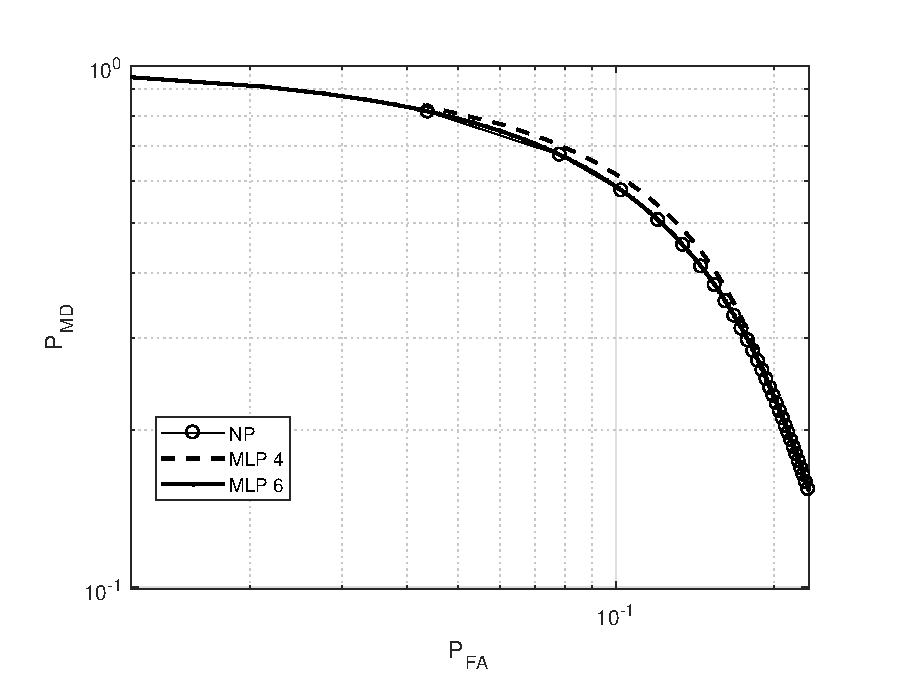
\includegraphics[width=1\columnwidth]{FA_MD_LOS.eps}
     \caption{\ac{md} probability vs. the \ac{fa} probability of the \ac{mlp} and of the optimal classificator. The number that follows \ac{mlp} indicates the number of neurons in the hidden layer.}
     \label{fig:NP_comp}
 \end{figure}


\subsection{Non-LOS Case}
We here consider a network with $N_{\rm BS}=5$ \acp{bs}, each one gathering attenuation values of \ac{ue} transmitted signal and collect them in the attenuation vector $\bm{a}$. Each \ac{bs} is characterized by different attenuation and shadowing map. Figure \ref{fig:trueMap} shows a realization of the path loss and shadowing map for a \ac{bs} located at the center of area $\mathcal{A}$. We further assume that within $\mathcal{A}$ are present two orthogonal \ac{los} paths traversing the center of $\mathcal{A}$. We define the legitimate area as the one contoured by the red line.


\begin{figure}[t]
    \centering
    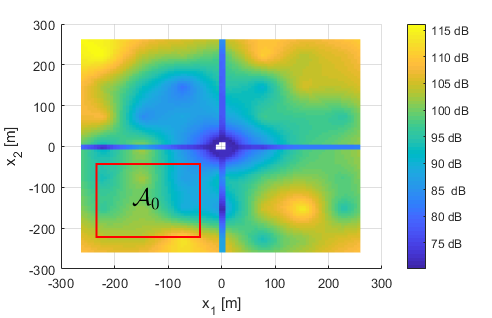
\includegraphics[width=1\columnwidth]{surfColorato.png}
    \caption{Example of a realization of the attenuation map in the non-\ac{los} scenario considering only the shadowing effects.}
    \label{fig:trueMap}
\end{figure}

Given many realization of the maps for all the $N_{\rm BS}$ we can compute the average \ac{fa} and \ac{md} probabilities of the authentication system.

Fig. \ref{fig:n_train} shows the average \ac{md} vs. \ac{fa} probabilities of the authentication system trained with $n_{train} = 10, 100, 1000$ and $10000$ points. We see that as the number of training points increases the average performance of the system increase.

\begin{figure}[t]
    \centering
    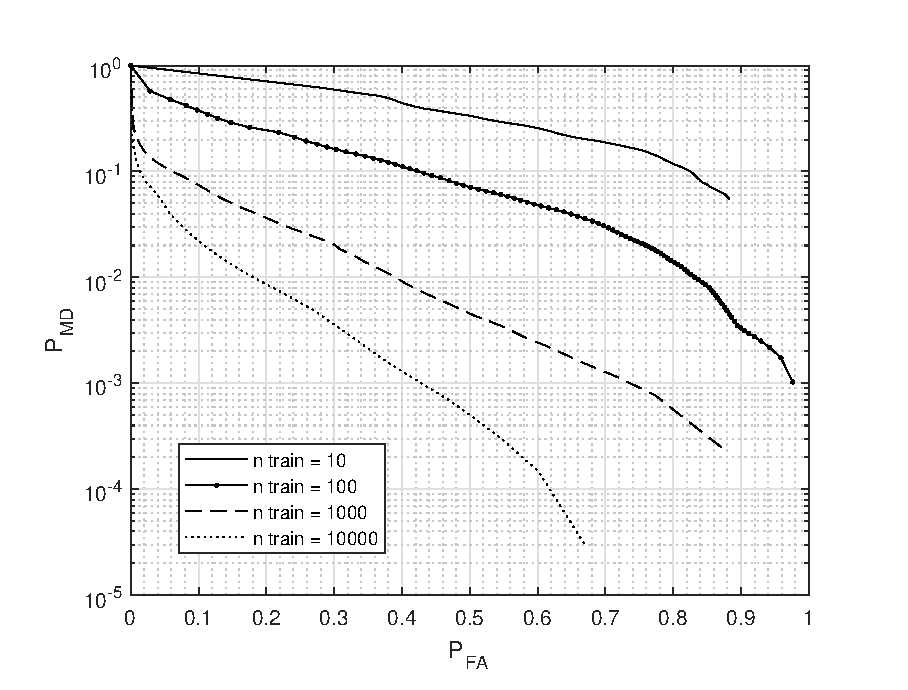
\includegraphics[width=1\columnwidth]{mean_maps.eps}
    \caption{Average \ac{md} vs. average \ac{fa} probabilities of the authentication system trained with different number of attenuation vectors.}
    \label{fig:n_train}
\end{figure}

\subsection{BSs Positioning}
We here consider the optimization Algorithm shown in Algorithm 1. We consider a \ac{pso} with $P=6$ particles, each composed by a set of $N_{\rm BS}=5$ \acp{bs} initialized with random positions. We initialize the parameters of the \ac{pso}, i.e., the inertia coefficient and the acceleration constants with the typical values $w=0.7298$, $c_1=c_2=1.4961$ \cite{Kennedy-11}. We consider different realizations of the shadowing map and obtained results are averaged over this realization. We consider a training set composed by $10^4$ points and a testing set of $10^3$ points.

Fig. \ref{fig:CE} shows the average \ac{ce} obtained by the global best particle vs. the considered \ac{pso} iteration. We see that as particles move the average \ac{ce} values decreases.

Fig. \ref{fig:CEvsAUC} shows the average \ac{auc} value vs. the number of iterations. In particular Fig. \ref{fig:CEvsAUC} compares the average \ac{auc} value obtained by training different \acp{nn} for each particle and optimizing the \ac{auc} with the \ac{auc} that would be obtained if testing the \ac{nn} that guarantees minimum \ac{ce}. We see that the \ac{auc} of the minimum \ac{ce} network is close to the one obtained by the minimum \ac{auc} network. This confirms our intuition that the \ac{ce} can be used as a proxy for the \ac{auc} and that \ac{pso} can be implemented without testing each \ac{nn} that would be needed for the different particles and their positions.

\begin{figure}[t]
    \centering
    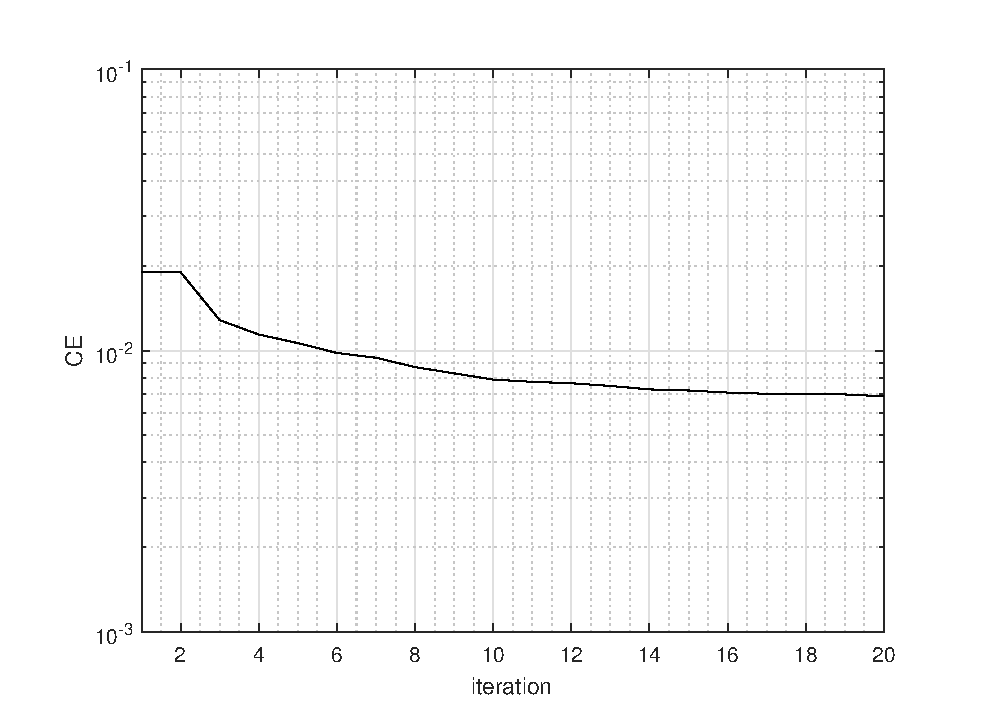
\includegraphics[width=1\columnwidth]{CE_71_real.eps}
    \caption{Mean \ac{ce} vs. number of \ac{pso} iterations.}
    \label{fig:CE}
\end{figure}

\begin{figure}[t]
    \centering
    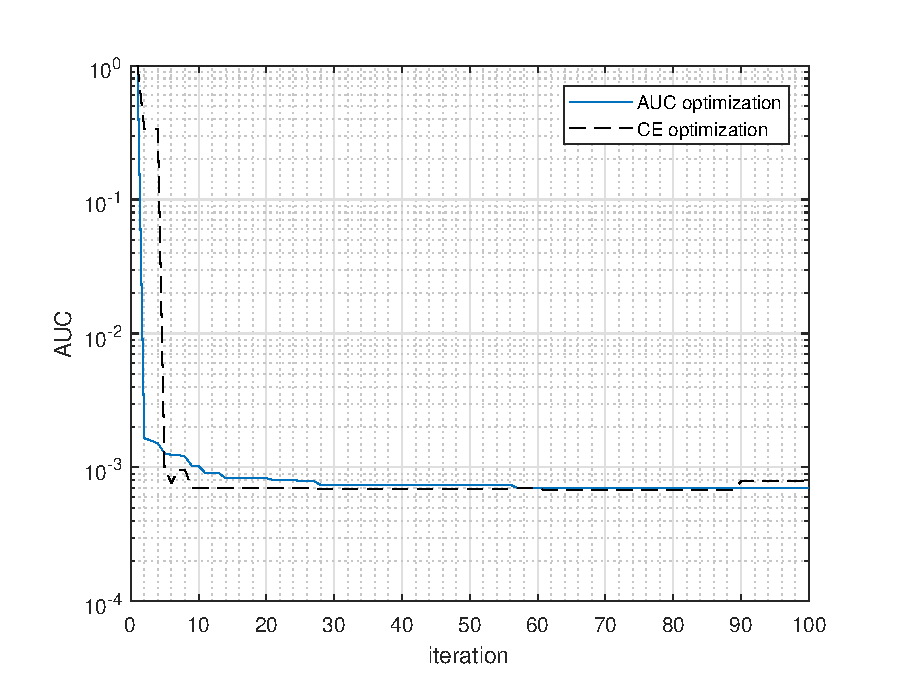
\includegraphics[width=1\columnwidth]{CE_vsAUC.eps}
    \caption{Mean \ac{auc} vs. number of \ac{pso} iterations. Comparison between the \ac{auc} obtained with testing and \ac{auc} obtained if testing the position that guarantees minimum \ac{ce}.}
    \label{fig:CEvsAUC}
\end{figure}

\section{Conclusions}

\renewcommand*{\bibfont}{\footnotesize}

\printbibliography
\balance
\end{document}
